% ==================================================================
% EBOOK ASAS PENDAWAIAN ELEKTRIK
% (Ringkasan Pendidikan – Bukan Dokumen Piawaian Rasmi)
% Versi 1.1
% ==================================================================
\documentclass[12pt,a4paper,oneside]{scrreprt}

% --------------------------------------------------
% Pakej asas & tipografi
% --------------------------------------------------
\usepackage[a4paper,margin=2.2cm]{geometry}
\usepackage{fontspec}
\setmainfont{Latin Modern Roman}
\setsansfont{Latin Modern Sans}
\setmonofont{Latin Modern Mono}
\usepackage{microtype}
\usepackage{setspace}
\onehalfspacing
\usepackage[dvipsnames,svgnames,x11names]{xcolor}
\usepackage{graphicx}
\usepackage{hyperref}
\hypersetup{
  colorlinks=true,
  linkcolor=MidnightBlue,
  urlcolor=RoyalBlue3,
  citecolor=BrickRed,
  pdfauthor={Nama Anda},
  pdftitle={Asas Pendawaian Elektrik},
  pdfsubject={Asas Pendawaian Elektrik - Pendidikan},
  pdfcreator={LaTeX},
  pdfkeywords={Pendawaian Elektrik, Suruhanjaya Tenaga, RCD, MCB, Keselamatan}
}
\usepackage{titlesec}
\titleformat{\chapter}{\normalfont\Huge\bfseries\color{MidnightBlue}}{\thechapter.}{0.7em}{}
\titleformat{\section}{\normalfont\Large\bfseries\color{RoyalBlue4}}{\thesection}{0.6em}{}
\titleformat{\subsection}{\normalfont\large\bfseries\color{RoyalBlue3}}{\thesubsection}{0.5em}{}

\usepackage{enumitem}
\setlist{topsep=4pt,itemsep=4pt,parsep=2pt}

\usepackage{array,booktabs,longtable,multirow}
\usepackage{siunitx}
\sisetup{detect-all, per-mode=symbol}

\usepackage{tcolorbox}
\tcbset{
  colback=White,
  colframe=RoyalBlue4,
  arc=2pt,
  left=6pt,right=6pt,top=6pt,bottom=6pt,
  boxsep=2pt
}

\usepackage{fancyhdr}
\pagestyle{fancy}
\fancyhf{}
\lhead{\textit{Asas Pendawaian Elektrik}}
\rhead{\thepage}
\renewcommand{\headrulewidth}{0.4pt}

\usepackage{tikz}
\usetikzlibrary{arrows.meta,positioning,calc,fit,shapes.misc,shapes.symbols,shapes.geometric}

\usepackage{amsmath,amssymb}

% --------------------------------------------------
% Warna tematik
% --------------------------------------------------
\definecolor{LiveColor}{HTML}{B34700}      % Coklat jingga (L)
\definecolor{NeutralColor}{HTML}{1F4E79}   % Biru gelap (N)
\definecolor{EarthColor}{HTML}{0A7D15}     % Hijau (E)
\definecolor{PanelGrey}{HTML}{DDDDDD}
\definecolor{AccentBlue}{HTML}{005F99}
\definecolor{WarnRed}{HTML}{C40000}
\definecolor{BackShade}{HTML}{F4F9FC}

% --------------------------------------------------
% Makro ringkas
% --------------------------------------------------
\newcommand{\Lwire}{\textcolor{LiveColor}{L}}
\newcommand{\Nwire}{\textcolor{NeutralColor}{N}}
\newcommand{\Ewire}{\textcolor{EarthColor}{E}}
\newcommand{\important}[1]{\textbf{\color{WarnRed}{#1}}}
\newcommand{\nota}[1]{\begin{tcolorbox}[colframe=AccentBlue,title=Nota Penting]#1\end{tcolorbox}}
\newcommand{\defbox}[2]{\begin{tcolorbox}[colframe=LiveColor,title={#1}]#2\end{tcolorbox}}
\newcommand{\contoh}[1]{\begin{tcolorbox}[colframe=NeutralColor,title=Contoh]#1\end{tcolorbox}}
\newcommand{\amaran}[1]{\begin{tcolorbox}[colframe=WarnRed,title=Amaran,colback=WarnRed!3]#1\end{tcolorbox}}

% --------------------------------------------------
% Tajuk dokumen
% --------------------------------------------------
\title{\vspace*{4cm}\Huge \textbf{ASAS PENDAWAIAN ELEKTRIK}\\[0.6em]
\Large (Ringkasan Pendidikan – Mengikut Amalan & Rujukan Piawaian Malaysia)}
\author{\Large Nama Anda\\[0.3em]
\small (Gantikan dengan nama penulis / organisasi)\\[0.5em]
\small E-mel: contoh@domain.com}
\date{\today}

% --------------------------------------------------
% Dokumen
% --------------------------------------------------
\begin{document}
\begin{titlepage}
\centering
{\color{RoyalBlue4}\rule{\linewidth}{1.2pt}}\\[1em]
{\Huge \textbf{ASAS PENDAWAIAN ELEKTRIK}}\\[0.7em]
{\Large (Ringkasan Pendidikan)}\\[1.2em]
{\large Versi 1.1}\\[2em]

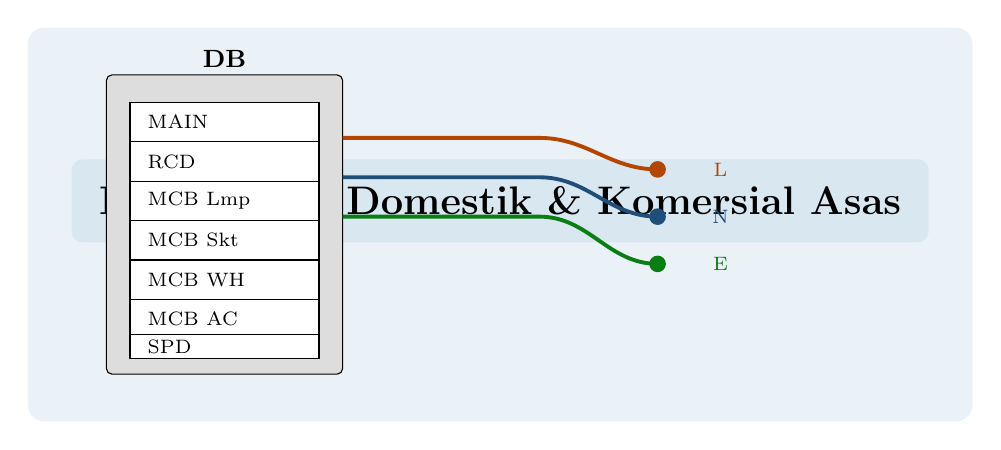
\begin{tikzpicture}[scale=1.0]
  \fill[AccentBlue!8,rounded corners=6pt] (0,0) rectangle (12,5);
  \node[rounded corners=4pt,fill=AccentBlue!15,inner sep=10pt] at (6,2.8){\Large \bfseries Pendawaian Domestik \& Komersial Asas};
  % Simbol ringkas papan agihan
  \draw[fill=PanelGrey,rounded corners=2pt] (1,0.6) rectangle (4,4.4);
  \node at (2.5,4.6){\small \textbf{DB}};
  \foreach \y/\lbl in {3.8/MAIN,3.3/RCD,2.8/MCB~Lmp,2.3/MCB~Skt,1.8/MCB~WH,1.3/MCB~AC} {
    \draw[fill=white] (1.3,\y-0.25) rectangle (3.7,\y+0.25);
    \node[anchor=west,font=\scriptsize] at (1.4,\y){\lbl};
  }
  \draw[fill=white] (1.3,0.8) rectangle (3.7,1.1);
  \node[anchor=west,font=\scriptsize] at (1.4,0.95){SPD};
  % Kabel keluar
  \foreach \i/\col in {0/LiveColor,1/NeutralColor,2/EarthColor}{
    \draw[line width=1.4pt,color=\col] (4,3.6-0.5*\i) -- (6.5,3.6-0.5*\i)
    to[out=0,in=180] (8,3.2-0.6*\i);
    \fill[\col] (8,3.2-0.6*\i) circle (3pt);
  }
  \node[font=\scriptsize] at (8.8,3.2){\Lwire};
  \node[font=\scriptsize] at (8.8,2.6){\Nwire};
  \node[font=\scriptsize] at (8.8,2.0){\Ewire};
\end{tikzpicture}

\vfill
\textbf{Penulis:} Nama Anda \\
\textbf{Tarikh:} \today \\
\vspace{1em}
{\color{RoyalBlue4}\rule{\linewidth}{1.2pt}}\\
\vfill
\end{titlepage}

\pagenumbering{roman}

\chapter*{Penafian}
Dokumen ini untuk tujuan \textbf{pendidikan asas}. Ia \textbf{bukan} pengganti kepada:
\begin{itemize}
  \item Akta Bekalan Elektrik 1990 (Akta 447)
  \item Peraturan-Peraturan Elektrik semasa
  \item Piawaian Malaysia / MS IEC 60364 penuh
\end{itemize}
Rujuk naskhah rasmi Suruhanjaya Tenaga (ST), SIRIM atau penerbit berautoriti untuk teks piawaian terperinci. Segala pemasangan perlu dilakukan oleh orang kompeten bertauliah (Wireman / Chargeman / Electrician) mengikut perundangan Malaysia. Contoh, nilai dan ilustrasi di sini adalah indikatif.

\tableofcontents
\listoftables

\clearpage
\pagenumbering{arabic}

% ================================================================
\chapter{Pengenalan}
Pendawaian elektrik ialah sistem konduktor, perlindungan, kawalan dan aksesori yang memastikan tenaga elektrik diagihkan kepada beban dengan \textbf{selamat}, \textbf{boleh dipercayai}, dan \textbf{efisien}. 
\section{Objektif Utama}
\begin{enumerate}
  \item Keselamatan renjatan (perlindungan sentuhan langsung/tidak langsung)
  \item Pencegahan kebakaran (arus lebih, pemanasan kabel)
  \item Kebolehpercayaan dan ketersediaan bekalan
  \item Kejatuhan voltan terkawal
  \item Kebolehselenggaraan dan modulariti masa depan
\end{enumerate}

\nota{Reka bentuk sebenar memerlukan pengiraan arus beban, kapasiti kabel ($I_z$), arus gangguan, koordinasi MCB/RCD, dan dokumentasi litar.}

% ================================================================
\chapter{Prinsip Asas Elektrik}
\section{Kuantiti Asas}
\begin{description}
  \item[Voltan (V):] Perbezaan potensi elektrik.
  \item[Arus (I):] Aliran cas (Ampere).
  \item[Rintangan (R):] Halangan kepada arus; Hukum Ohm: $V = I R$.
  \item[Kuasa (P):] 1 fasa: $P = VI$; 3 fasa: $P \approx \sqrt{3} V_{LL} I \cos\phi$.
  \item[Tenaga (kWh):] Kuasa (kW) $\times$ masa (jam).
\end{description}

\section{Faktor Kuasa}
Faktor kuasa rendah meningkatkan arus dan rugi $I^2R$, menyebabkan pemanasan kabel dan kejatuhan voltan lebih tinggi.

\section{Contoh Pengiraan}
Beban 2 kW, $V=230$ V, pf $\approx 1$: $I \approx 2000/230 = 8.7$ A.  
Beban 4 kW, pf $=0.95$: $I \approx \frac{4000}{230 \times 0.95} \approx 18.4$ A.

% ================================================================
\chapter{Rangka Kerja Perundangan \& Piawaian}
\section{Rujukan}
\begin{itemize}
  \item Akta Bekalan Elektrik 1990
  \item Peraturan-Peraturan Elektrik
  \item MS IEC 60364 (adaptasi pemasangan bangunan)
  \item Garis panduan / circular Suruhanjaya Tenaga
\end{itemize}

\amaran{Teks piawaian rasmi dilindungi hak cipta. Dokumen ini hanya ringkasan pendidikan.}

% ================================================================
\chapter{Komponen Asas Pendawaian}
\section{Senarai Ringkas}
\begin{longtable}{p{3cm}p{10cm}}
\toprule
\textbf{Komponen} & \textbf{Fungsi} \\
\midrule
Kabel & Mengangkut arus (L, N, E) \\
MCB & Perlindungan arus lebih/pintas litar akhir \\
RCD (RCCB) & Perlindungan arus baki (kebocoran ke bumi) \\
MCCB & Perlindungan kapasiti lebih tinggi \\
Fuse & Perlindungan arus lebih (pakai sekali) \\
SPD & Lindungan lonjakan transien (petir/switching) \\
Suis & Putus/sambung litar beban \\
Soket 13A & Bekal peralatan mudah alih \\
Conduit/Trunking & Perlindungan mekanikal kabel \\
Earth/Neutral Bar & Pengurusan terminasi bumi/neutral \\
Contactor & Kawal litar kuasa melalui litar kawalan \\
Overload Relay & Perlindungan beban lampau motor \\
\bottomrule
\end{longtable}

% ================================================================
\chapter{Earthing \& Sistem Pembumian}
\section{Jenis Sistem}
Sistem lazim: TN-S, TN-C-S (PME), TT (khusus), IT (terasing, aplikasi khas).
\section{Tujuan Pembumian}
\begin{enumerate}
  \item Laluan arus gangguan yang pantas untuk operasi perlindungan.
  \item Menstabilkan voltan terhadap bumi.
  \item Mengurangkan risiko sentuhan bahaya.
\end{enumerate}

\section{Diagram TN-S (Ringkas TikZ)}
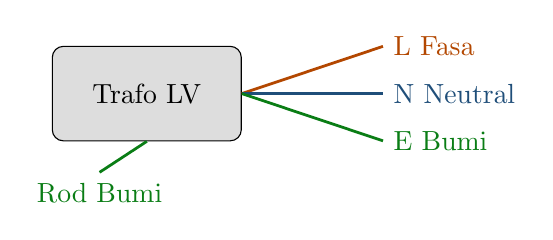
\begin{tikzpicture}[x=1.0cm,y=1.0cm]
  \node[draw,rounded corners,fill=PanelGrey,minimum width=2.4cm,minimum height=1.2cm] (tx) at (0,0){Trafo LV};
  \draw[line width=1pt,LiveColor] (tx.east) -- (3,0.6) node[right]{\Lwire ~Fasa};
  \draw[line width=1pt,NeutralColor] (tx.east) -- (3,0.0) node[right]{\Nwire ~Neutral};
  \draw[line width=1pt,EarthColor] (tx.east) -- (3,-0.6) node[right]{\Ewire ~Bumi};
  \draw[EarthColor,line width=1pt] (-0.6,-1.0) node[below]{Rod Bumi} -- (tx.south);
\end{tikzpicture}

% ================================================================
\chapter{Jenis Sistem Pendawaian}
\section{Kaedah Pemasangan}
\begin{itemize}
  \item Conduit tertanam (concealed)
  \item Conduit permukaan (PVC / galvanised)
  \item Trunking \& cable tray (komersial)
  \item Kabel berperisai (SWA) luar / mekanikal kuat
  \item Pendawaian fleksibel untuk sambungan peralatan mudah alih
\end{itemize}

% ================================================================
\chapter{Perlindungan Litar}
\section{Peranti}
\begin{description}
  \item[MCB:] Kurva B,C,D – arus lebih \& pintas.
  \item[MCCB:] Boleh laras tetapan trip; arus lebih tinggi.
  \item[RCD 30 mA:] Perlindungan hayat.
  \item[RCD 100/300 mA:] Perlindungan kebakaran kumpulan.
  \item[SPD:] Lindungan lonjakan (surge).
\end{description}

\section{Rangkaian Perlindungan (TikZ)}
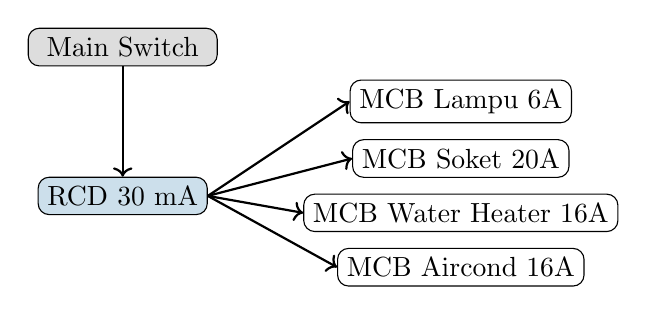
\begin{tikzpicture}[node distance=1.4cm]
  \node[draw,rounded corners,fill=PanelGrey,minimum width=2.4cm] (main){Main Switch};
  \node[draw,rounded corners,fill=AccentBlue!20,below=of main] (rcd){RCD 30 mA};
  \node[draw,rounded corners,fill=white,right=1.8cm of rcd,yshift=1.2cm] (m1){MCB Lampu 6A};
  \node[draw,rounded corners,fill=white,below=0.2cm of m1] (m2){MCB Soket 20A};
  \node[draw,rounded corners,fill=white,below=0.2cm of m2] (m3){MCB Water Heater 16A};
  \node[draw,rounded corners,fill=white,below=0.2cm of m3] (m4){MCB Aircond 16A};
  \draw[->,thick] (main) -- (rcd);
  \foreach \x in {m1,m2,m3,m4}{
    \draw[->,thick] (rcd.east) -- (\x.west);
  }
\end{tikzpicture}

% ================================================================
\chapter{Reka Bentuk Litar Asas}
\section{Litar Lampu Satu Suis}
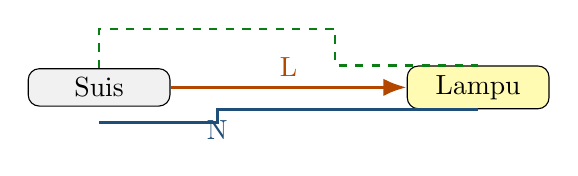
\begin{tikzpicture}
  \node[draw,rounded corners,minimum width=1.8cm,fill=PanelGrey!40] (sw){Suis};
  \node[draw,rounded corners,minimum width=1.8cm,fill=yellow!30,right=3cm of sw] (lp){Lampu};
  \draw[LiveColor,very thick,-{Latex}] (sw) -- (lp) node[midway,above]{L};
  \draw[NeutralColor,very thick] ($(sw.south)+(0,-0.2)$) -- ++(1.5,0) |- (lp.south) node[midway,below]{N};
  \draw[EarthColor,thick,dashed] (sw.north) -- ++(0,0.5) -- ++(3,0) |- (lp.north);
\end{tikzpicture}

\section{Litar Soket: Radial vs Ring}
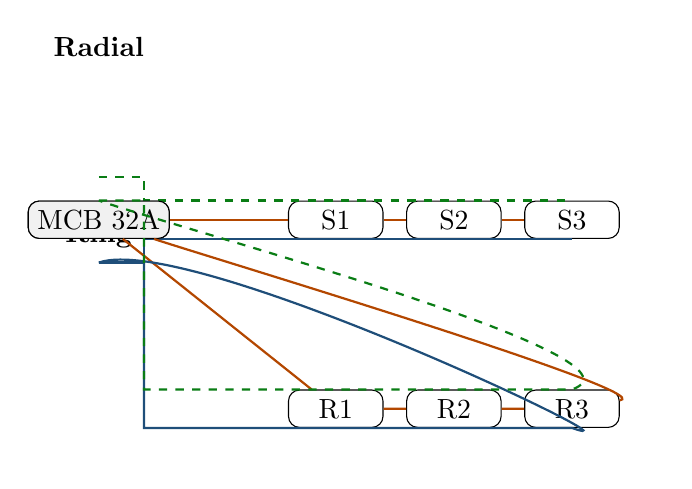
\begin{tikzpicture}[x=1.15cm,y=1cm]
  % Radial
  \node at (0,2.2){\textbf{Radial}};
  \node[draw,rounded corners,fill=PanelGrey!40,minimum width=1.5cm] (mrad){MCB 20A};
  \foreach \i in {1,2,3}{
    \node[draw,rounded corners,fill=white,minimum width=1.2cm,right=1.5*\i cm of mrad] (s\i){S\i};
  }
  \draw[LiveColor,thick] (mrad) -- (s1) -- (s2) -- (s3);
  \draw[NeutralColor,thick] ($(mrad.south)+(0,-0.3)$) -- ++(0.5,0) |- (s1.south) -- (s2.south) -- (s3.south);
  \draw[EarthColor,thick,dashed] ($(mrad.north)+(0,0.3)$) -- ++(0.5,0) |- (s1.north) -- (s2.north) -- (s3.north);

  % Ring
  \node at (0,-0.2){\textbf{Ring}};
  \node[draw,rounded corners,fill=PanelGrey!40,minimum width=1.5cm] (mring){MCB 32A};
  \foreach \i in {1,2,3}{
    \node[draw,rounded corners,fill=white,minimum width=1.2cm,right=1.5*\i cm of mring,yshift=-2.4cm] (r\i){R\i};
  }
  \draw[LiveColor,thick] (mring) -- (r1) -- (r2) -- (r3) .. controls +(1,0.2) and +(1,-0.4) .. (mring);
  \draw[NeutralColor,thick] ($(mring.south)+(0,-0.3)$) -- ++(0.5,0) |- (r1.south) -- (r2.south) -- (r3.south)
    .. controls +(1,-0.4) and +(1,0.4) .. ($(mring.south)+(0,-0.3)$);
  \draw[EarthColor,thick,dashed] (mring.north) -- ++(0.5,0) |- (r1.north) -- (r2.north) -- (r3.north)
    .. controls +(1,0.4) and +(1,-0.4) .. (mring.north);
\end{tikzpicture}

\section{Litar Motor Kecil (Contactor + Overload)}
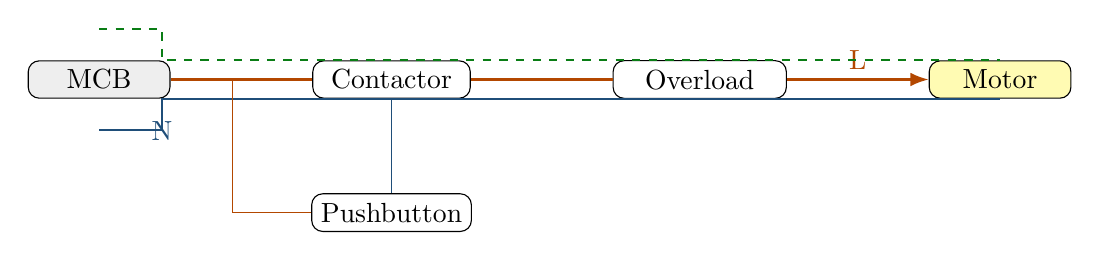
\begin{tikzpicture}[node distance=1.8cm]
  \node[draw,rounded corners,fill=PanelGrey!50,minimum width=1.8cm] (mcb){MCB};
  \node[draw,rounded corners,fill=white,minimum width=2.0cm,right=of mcb] (cont){Contactor};
  \node[draw,rounded corners,fill=white,minimum width=2.2cm,right=of cont] (ol){Overload};
  \node[draw,rounded corners,fill=yellow!30,minimum width=1.8cm,right=of ol] (mot){Motor};
  \draw[LiveColor,thick,-{Latex}] (mcb) -- (cont) -- (ol) -- (mot) node[midway,above]{L};
  \draw[NeutralColor,thick] ($(mcb.south)+(0,-0.4)$) -- ++(0.8,0) |- (mot.south) node[pos=0.3,below]{N};
  \draw[EarthColor,thick,dashed] ($(mcb.north)+(0,0.4)$) -- ++(0.8,0) |- (mot.north);
  % Coil control simplified
  \node[draw,rounded corners,fill=white,below=1.2cm of cont] (sw){Pushbutton};
  \draw[NeutralColor,thin] (sw) -- (cont.south);
  \draw[LiveColor,thin] (sw.west) -- ++(-1,0) |- (cont.west);
\end{tikzpicture}

% ================================================================
\chapter{Saiz Kabel \& Faktor Pembetulan}
\section{Langkah Umum}
\begin{enumerate}
  \item Tentukan arus reka bentuk $I_b$.
  \item Pilih MCB ($I_n \ge I_b$ dan $I_n \le I_z$).
  \item Semak jatuhan voltan $\Delta V$ (dalam had).
  \item Aplikasikan faktor pembetulan (suhu, kumpulan kabel, kaedah pemasangan).
  \item Sahkan koordinasi perlindungan dan masa trip.
\end{enumerate}

\section{Faktor Pembetulan Tipikal (Ringkas)}
\begin{itemize}
  \item Suhu persekitaran lebih tinggi → keupayaan arus turun.
  \item Pengelompokan banyak kabel → keupayaan arus turun.
  \item Kaedah pemasangan (dalam penebat vs terbuka) mempengaruhi penyejukan.
\end{itemize}

\section{Contoh}
Beban 4 kW, 230 V, pf $=0.95$: $I_b \approx 18.4$ A. Jika faktor derating gabungan $=0.8$, arus efektif untuk pemilihan kabel $= 18.4 / 0.8 \approx 23$ A → pilih kabel dengan $I_z$ lebih tinggi (misalnya 4 mm$^2$ jika 2.5 mm$^2$ tidak mencukupi mengikut jadual standard).

% ================================================================
\chapter{Papan Agihan (Distribution Board)}
\section{Contoh Susun Atur}
\begin{tcolorbox}
Main Isolator $\rightarrow$ SPD $\rightarrow$ RCCB 63A/30mA $\rightarrow$
\begin{itemize}
  \item MCB 6A Lampu
  \item MCB 20A Soket Radial
  \item MCB 32A Ring Soket
  \item MCB 16A Aircond
  \item MCB 16A Water Heater
\end{itemize}
\end{tcolorbox}

\section{Aspek Penting}
\begin{itemize}
  \item Label jelas setiap litar
  \item Ruang lebihan (spare ways) untuk masa depan
  \item Penyelenggaraan: terminal ketat, tiada discoloration
\end{itemize}

% ================================================================
\chapter{Simbol (Ringkasan)}
\begin{tabular}{ll}
\toprule
Simbol & Maksud\\
\midrule
\Lwire & Live (Fasa) \\
\Nwire & Neutral \\
\Ewire & Bumi \\
MCB & Miniature Circuit Breaker \\
RCD & Residual Current Device \\
(DB) & Distribution Board \\
SPD & Surge Protective Device \\
\bottomrule
\end{tabular}

% ================================================================
\chapter{Prosedur Kerja Selamat}
\section{Langkah Umum}
\begin{enumerate}
  \item Perancangan: semak lukisan terkini
  \item Isolasi bekalan (LOTO)
  \item Uji ketiadaan voltan (test-before-touch)
  \item Laksanakan kerja dengan PPE sesuai
  \item Ujian semula dan energize berperingkat
\end{enumerate}

\section{PPE}
Sarung tangan bertebat, kasut keselamatan, pelindung mata, pakaian kapas, peralatan pengesan voltan sah.

\amaran{Jangan bekerja pada litar hidup tanpa prosedur kerja selamat khusus dan kebenaran.}

% ================================================================
\chapter{Ujian \& Pemeriksaan}
\section{Urutan Lazim}
\begin{enumerate}
  \item Pemeriksaan visual
  \item Continuity CPC
  \item Insulation resistance
  \item Polariti
  \item Earth fault loop impedance
  \item Ujian RCD (masa trip)
  \item Ujian fungsi (operasi beban, suis)
\end{enumerate}

\section{Jadual Ringkas Ujian}
\begin{longtable}{p{3.2cm}p{5.5cm}p{4.5cm}}
\toprule
Ujian & Tujuan & Alat \\
\midrule
Continuity CPC & Laluan bumi lengkap & Ohmmeter \\
Insulation Resistance & Penebatan memadai & IR Tester (Megger) \\
Polariti & Suis putuskan fasa (bukan neutral) & Multimeter \\
Earth Loop & Pastikan masa trip perlindungan & Loop tester \\
RCD Trip & Keselamatan hayat / kebakaran & RCD tester \\
\bottomrule
\end{longtable}

% ================================================================
\chapter{Penyelenggaraan}
\section{Aktiviti Berkala}
\begin{itemize}
  \item Ketatkan semula terminal (jika longgar)
  \item Ujian butang RCD bulanan
  \item Pemeriksaan discoloration / bau hangit
  \item Rekod pengukuran dan tarikh
\end{itemize}

\section{Rekod}
Simpan log: tarikh, litar diuji, nilai pengukuran, tindakan pembetulan.

% ================================================================
\chapter{Latihan Soalan}
\begin{enumerate}
  \item Jelaskan fungsi RCD 30 mA.
  \item Bezakan litar radial dan ring.
  \item Mengapa continuity CPC diuji?
  \item Apakah faktor asas dalam pemilihan saiz kabel?
  \item Nyatakan langkah asas LOTO.
  \item Apakah tujuan SPD?
  \item Berikan contoh pengiraan arus bagi beban 3 kW, 230 V, pf=0.9.
\end{enumerate}

\section{Contoh Jawapan Ringkas}
\begin{itemize}
  \item[(1)] Perlindungan arus baki kecil (renjatan).
  \item[(2)] Radial hujung buntu; ring kembali semula ke MCB (dua laluan).
  \item[(3)] Menjamin laluan bumi rendah impedans untuk operasi perlindungan.
  \item[(4)] $I_b$, faktor derating, jatuhan voltan, koordinasi perlindungan.
  \item[(5)] Isolasi, kunci/tag, uji tiada voltan, kerja selamat, pulih bekalan.
  \item[(6)] Lindung lonjakan transien.
  \item[(7)] $I = \frac{3000}{230 \times 0.9} \approx 14.5$ A.
\end{itemize}

% ================================================================
\chapter{Glosari Ringkas}
\begin{tabular}{p{3cm}p{10cm}}
\toprule
Istilah & Definisi \\
\midrule
CPC & Circuit Protective Conductor \\
Loop Impedance & Impedans laluan arus gangguan ke sumber \\
PME & Protective Multiple Earthing (TN-C-S) \\
Voltage Drop & Pengurangan voltan sepanjang kabel \\
Derating & Pengurangan kapasiti arus kabel kerana kondisi pemasangan \\
Fault Current & Arus sangat tinggi ketika pintas (short circuit) \\
Trip Curve & Hubungan masa–arus bagi MCB \\
\bottomrule
\end{tabular}

% ================================================================
\chapter{Rujukan}
\begin{itemize}
  \item Suruhanjaya Tenaga Malaysia – \url{https://www.st.gov.my/}
  \item Akta Bekalan Elektrik 1990
  \item MS IEC 60364 (Rujukan pemasangan bangunan)
  \item Garis panduan keselamatan kerja elektrik (amalan industri)
\end{itemize}

% ================================================================
\appendix
\chapter{Lampiran: Templat Rekod Ujian}
\begin{longtable}{p{1.4cm}p{1.5cm}p{1.2cm}p{1.5cm}p{1.8cm}p{1.8cm}p{1.5cm}p{1.6cm}p{2cm}}
\toprule
Litar & Jenis & MCB(A) & Kabel(mm$^2$) & Cont. (Ω) & IR (MΩ) & Loop (Ω) & RCD (ms) & Catatan \\
\midrule
\endhead
\bottomrule
\end{longtable}

\chapter{Lampiran: Nota Tambahan}
Anda boleh menambah:
\begin{itemize}
  \item Kecekapan Tenaga
  \item Integrasi PV asas (perlindungan, anti-islanding ringkas)
  \item Automasi pintar (sensor, relay pintar)
\end{itemize}

\vfill
\begin{center}
\textit{Tamat Dokumen}
\end{center}

\end{document}
